The Deployment Diagram shown below describes how the logical components designed in the context of the Component Diagram are to be physically deployed on the different devices needed for the functioning of the system.

As shown, the app server hosts the main logic components and manages their interaction. It provides access to them through the APIs defined in \autoref{sec:components_interfaces} and guarantees they can access the data layer residing on the database server.\newline
Every client with a significant application layer implements a limited subset of components responsible to interpret the inputs from the users and perform requests to the app server. When needed, an apposite module for the localization is included as well.\newline
The web server provides static web pages and the logic necessary to the browser to interact with the app server.

\begin{sidewaysfigure}
	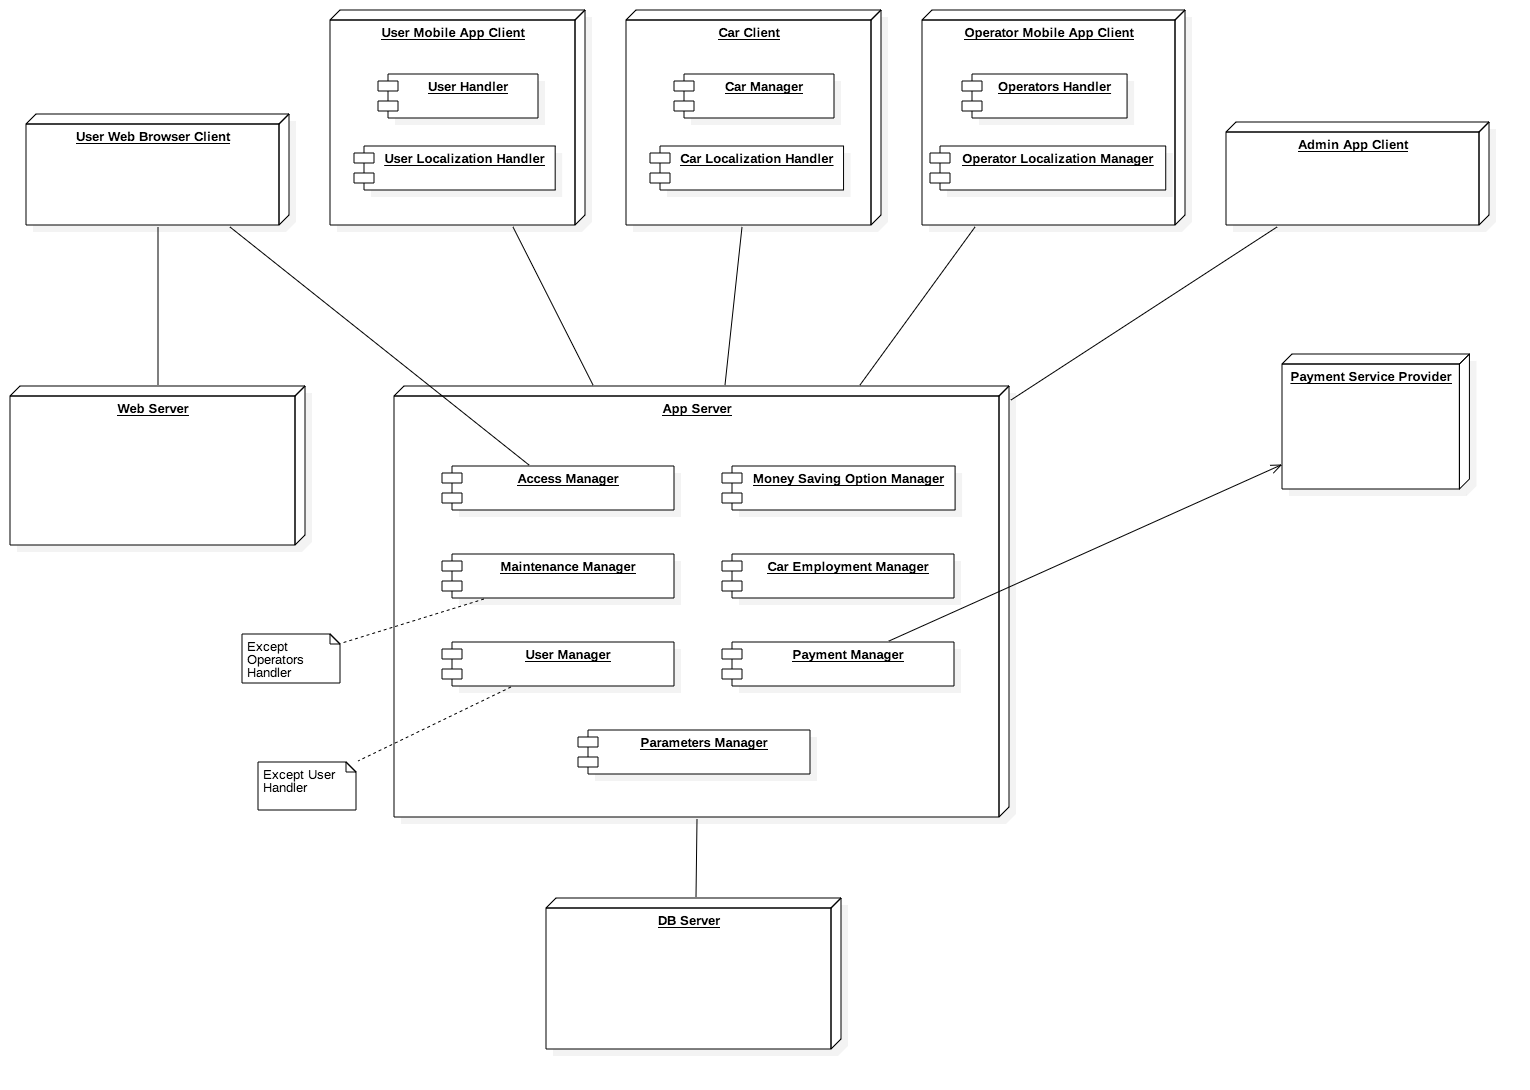
\includegraphics[width=\hsize, center]{img/deployment_diagrams/global.png}
\end{sidewaysfigure}

	\subsubsection{Non functional requirements}
		The architectural structure proposed addresses the non-functional requirements of \textit{integrity} and \textit{confidentiality} (see RASD) introducing a DMZ which separates with a firewall the app server, accessible from the outside network, from the database server. To avoid intrusions on the app server, another firewall is provided, with less restricting rules to allow outside clients to access. This way, even if an attack is performed to the app server, a more impenetrable layer of security still divides the intruders from the sensitive data. The structure just described is a standard pattern in the design of three-layer architectures.

		The app server is designed as a distributed system completely replicated in at least another physical machine, to fulfil the requirement of \textit{availabilty} and partially address the requirement of \textit{performance} (see RASD). A load balancer is expected to redirect the workload to the appropriate physical server. The number of servers can be increased in future if the workload requires it. This structure, along with a proper firewall configuration, helps to reduce the risk of failure for DOS attacks.

		Internally, each physical server is implemented following the \textit{elasticity pattern}, to fulfil the requirement of \textit{performance} (see RASD) while maintaining the number of allocated resources low. Thus, the components are to be instantiated according to the present load of clients' requests. An \textit{elastic load balancer} is used to manage the scaling process.

		To address the requirement of \textit{robustness} (see RASD) a simple error handling in the client application is enough. However, given the importance of failure management to avoid damages or theft to be performed to the cars, the data layer is chosen to be distributed.

		Lastly, the modularization of components and the possibility for the administrators to modify the core parameters of the system through the \textit{Parameters Manager} is conform to the \textit{design for flexibility} principle and satisfies the non-functional requirement of \textit{flexibility} (see RASD).
\FloatBarrier

% TODO talk about technological choices for APIs, app server, db server, mobile apps, desktop apps, browser, ...

% TODO provide physical diagram with distribution and platforms
